\chapter{Iterazione 2}

\section{Introduzione}
Nella seconda iterazione si è deciso di implementare i seguenti casi d'uso:

\begin{itemize}
    \item UC1 Prenotazioni [Astratto]
    \begin{itemize}
        \item UC1.1 Nuova prenotazione
        \item UC1.2 Visualizzazione prenotazioni
        \item UC1.3 Modifica prenotazione
        \item UC1.4 Elimina prenotazione
    \end{itemize}
    \item UC2 Algoritmo barche ed escursioni
\end{itemize}

Seguono una descrizione testuale di questi casi e i diagrammi dei componenti e di deployment.

\section{UC1: Prenotazioni}
\emph{Breve descrizione}: L'utente, dopo essersi loggato, può effettuare la prenotazione per una delle escursioni organizzate dal proprietario. Gli è possibile prenotare un posto non solo per sé stesso ma anche per altre persone, indicando il numero di partecipanti totale. Oltre alla creazione di una prenotazione, l'utente deve poter visualizzare le prenotazioni effettuate ed eventualmente modificarle o eliminarle.
Il caso d'uso Prenotazioni è suddiviso in 4 casi d'uso concreti:

\begin{itemize}
    \item UC1.1 Visualizzazione prenotazioni 
    \item UC1.2 Nuova prenotazione
    \item UC1.3 Modifica prenotazione
    \item UC1.4 Elimina prenotazione
\end{itemize}

\noindent \emph{Attori coinvolti}: Utente, Sistema.\medbreak
\noindent \emph{Trigger}: login dell'utente avvenuto con successo.\medbreak
\noindent \emph{Postcondizione}: l'utente dopo il login viene indirizzato alla home page e può scegliere se cliccare uno dei bottoni: Nuova prenotazione o Visualizza prenotazioni.\medbreak
\noindent \emph{Procedimento}:
\begin{enumerate}
    \item l'utente effettua il login
    \item Il sistema mostra la pagina iniziale che comprende i bottoni Visualizza e Nuova Prenotazione con cui l'utente può gestire le sue prenotazioni.
\end{enumerate}

\subsection{UC1.1 Visualizzazione prenotazioni}
\noindent \emph{Breve descrizione}: L'utente visualizza le prenotazioni effettuate e i relativi dati.\medbreak
\noindent \emph{Attori coinvolti}: Utente, Sistema.\medbreak
\noindent \emph{Trigger}: L'utente clicca il bottone Visualizza.\medbreak
\noindent \emph{Postcondizione}: Il sistema mostra una vista con l'elenco delle prenotazioni.\medbreak
\noindent \emph{Procedimento}:

\begin{enumerate}
    \item L'utente effettua il login
    \item L'utente clicca il bottone Visualizza presente nella home page.
    \item Il sistema mostra l'elenco delle prenotazioni presenti nel database a suo nome con le seguenti informazioni:
    \begin{itemize}
        \item id prenotazione
        \item id escursione
        \item data e ora escursione
        \item numero di persone per cui si è prenotato
        \item disposizione persone sulle barche (idbarca e numPersone)
    \end{itemize}
    \item Per ogni item dell'elenco l'utente può cliccare su Modifica prenotazione o Elimina prenotazione
\end{enumerate}

\subsection{UC1.2 Nuova prenotazione}
\noindent \emph{Breve descrizione}: L'utente effettua una nuova prenotazione per un'escursione organizzata dal proprietario.\medbreak
\noindent \emph{Attori coinvolti}: Utente, Sistema.\medbreak
\noindent \emph{Trigger}: L'utente clicca il bottone Nuova prenotazione.\medbreak
\noindent \emph{Postcondizione}: Il sistema mostra la nuova prenotazione all'interno della pagina di visualizzazione delle prenotazioni.\medbreak
\noindent \emph{Procedimento}:

\begin{enumerate}
    \item L'utente si trova sulla home page e clicca il bottone Nuova prenotazione.
    \item Il sistema mostra un form in cui è possibile specificare i dati relativi alla prenotazione.
    \item L'utente riempie il form e clicca il pulsante Conferma.
    \item Il sistema mostra la prenotazione effettuata all'interno della pagina di visualizzazione delle prenotazioni.
\end{enumerate}

\subsection{UC1.3 Modifica prenotazione}
\noindent \emph{Breve descrizione}: L'utente si trova sulla pagina di visualizzazione delle prenotazioni e clicca sul bottone Modifica di una di queste. Tale modifica può essere effettuata per aumentare o ridurre il numero di persone legate alla prenotazione (possibile fino a 3gg prima dell'escursione).\medbreak
\noindent \emph{Attori coinvolti}: Utente, Sistema.\medbreak
\noindent \emph{Trigger}: L'utente clicca su un bottone Modifica prenotazione.\medbreak
\noindent \emph{Postcondizione}: Il sistema mostra la prenotazione modificata all'interno della pagina di visualizzazione delle prenotazioni.\medbreak
\noindent \emph{Procedimento}:

\begin{enumerate}
    \item L'utente si trova sulla pagina di visualizzazione delle prenotazioni e clicca su un bottone Modifica.
    \item Il sistema mostra una vista in cui è possibile modificare i dati relativi alla prenotazione.
    \item L'utente modifica i dati e clicca su Conferma.
    \item Il sistema mostra la prenotazione aggiornata all'interno della pagina di visualizzazione delle prenotazioni.
\end{enumerate}

\subsection{UC1.4 Elimina prenotazione}
\noindent \emph{Breve descrizione}: L'utente si trova sulla pagina di visualizzazione delle prenotazioni e clicca sul bottone Elimina di una di queste. Dopo aver confermato la scelta, la prenotazione viene eliminata definitivamente.\medbreak
\noindent \emph{Attori coinvolti}: Utente, Sistema.\medbreak
\noindent \emph{Trigger}: L'utente clicca su un bottone Elimina prenotazione.\medbreak
\noindent \emph{Postcondizione}: Il sistema mostra la pagina di visualizzazione delle prenotazioni in cui non comparirà la prenotazione eliminata.\medbreak
\noindent \emph{Procedimento}:

\begin{enumerate}
    \item L'utente si trova sulla pagina di visualizzazione delle prenotazioni e clicca su un bottone Elimina.
    \item Il sistema mostra una finestra di dialogo per chiedere conferma.
    \item L'utente clicca su Conferma o Annulla.
    \item In caso di conferma il sistema mostra la pagina di visualizzazione delle prenotazioni senza la prenotazione appena eliminata.
\end{enumerate}

\section{UC2: Algoritmo barche ed escursioni}
\noindent \emph{Breve descrizione}: L'utente ha richiesto di effettuare una prenotazione specificando l'escursione e il numero di persone nel proprio gruppo. Il sistema deve allocare in modo ottimale sulle barche i posti appena richiesti e quelli di altri utenti già prenotati. Lo scopo dell'algoritmo è quello di minimizzare il numero di barche impiegate per l'escursione, così da ridurre i costi del proprietario, e cercare di non separare i gruppi.\medbreak
\noindent \emph{Attori coinvolti}: Utente, Sistema.\medbreak
\noindent \emph{Trigger}: L'utente conferma la richiesta di prenotazione.\medbreak
\noindent \emph{Postcondizione}: La disposizione dei posti dell'escursione è stata aggiornata e l'utente riceve una conferma di prenotazione.\medbreak
\noindent \emph{Procedimento}:

\begin{enumerate}
    \item L'utente clicca su conferma prenotazione.
    \item Il sistema esegue l'algoritmo di allocazione. Viene osservata la disposizione attuale dei gruppi:
    \begin{itemize}
        \item Se il numero di posti liberi è minore delle persone del nuovo gruppo viene allocata una nuova barca
        \item Se possibile, il gruppo viene allocato interamente su una delle barche già presenti
        \item ...
    \end{itemize}
    \item La nuova disposizione viene aggiornata nel database
    \item Viene mandata una conferma di prenotazione all'utente.
\end{enumerate}

\section{UML Component Diagram}
I casi d’uso scelti in questa prima iterazione vengono rappresentati sottoforma di componenti nel diagramma in Figura Figura~\ref{fig:componentDiagram2}. Come per l'iterazione precedente, si è scelto di suddividire i casi d’uso in componenti boundary, control e data.

\begin{figure}[!ht]
    \centering
    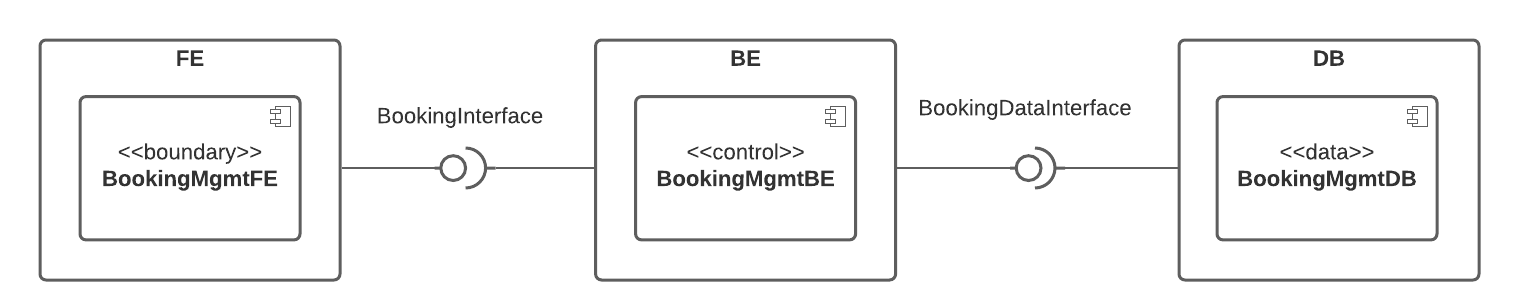
\includegraphics[width=\textwidth]{ComponentDiagram2_v1.png}
    \caption{Diagramma dei componenti UML.}\label{fig:componentDiagram2}
\end{figure}

\section{UML Class Diagram per Interfacce}
Il diagramma in Figura ~\ref{fig:ClassDiagramInterfaces2} serve a rappresentare le interfacce del sistema e le
loro interazioni.

\begin{figure}[!ht]
    \centering
    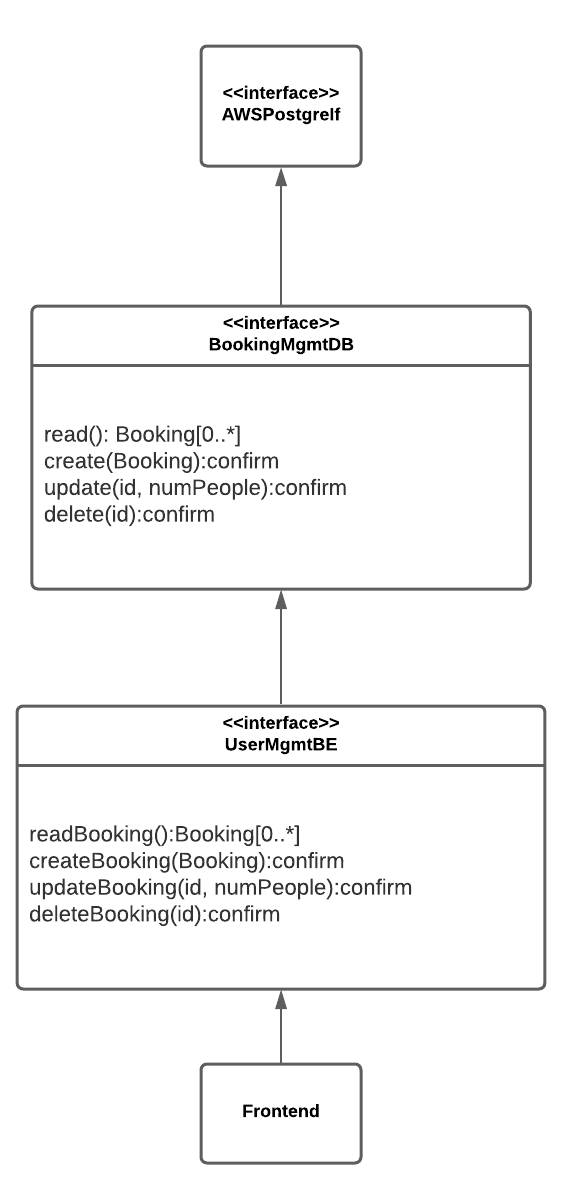
\includegraphics{ClassDiagramInterfaces2_v1.png}
    \caption{Diagramma delle classi per interfacce UML.}\label{fig:ClassDiagramInterfaces2}
\end{figure}

\section{UML Class diagram per tipi di dato}
Il tipo Booking è stato già esplicitato nell'iterazione precedente nel Class diagram per tipi di dato.
Viene riportato di seguito in Figura ~\ref{fig:BookingType}.

\begin{figure}[!ht]
    \centering
    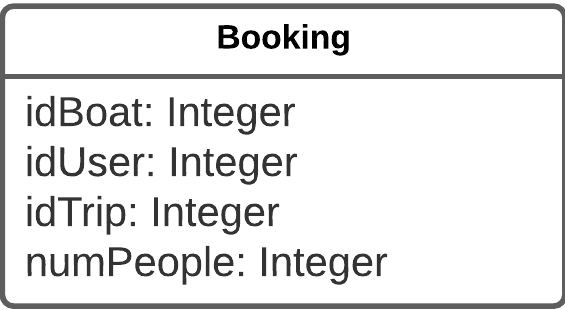
\includegraphics[scale=0.4]{booking.png}
    \caption{Tipo di dato Booking}\label{fig:BookingType}
\end{figure}

\section{UML Deployment diagram}
I componenti descritti precedentemente vengono istanziati nel Deployment diagram.
In Figura ~\ref{fig:DeploymentDiagram2} vengono mostrati i componenti contenuti nei seguenti nodi:
\begin{itemize}
    \item Cellulare utente è il nodo su cui una persona potrà gestire le prenotazioni.
    \item Web server fornisce le API richieste dall’applicativo lato front-end.
    \item Database funge da storage dei dati.
\end{itemize}

\begin{figure}[!ht]
    \centering
    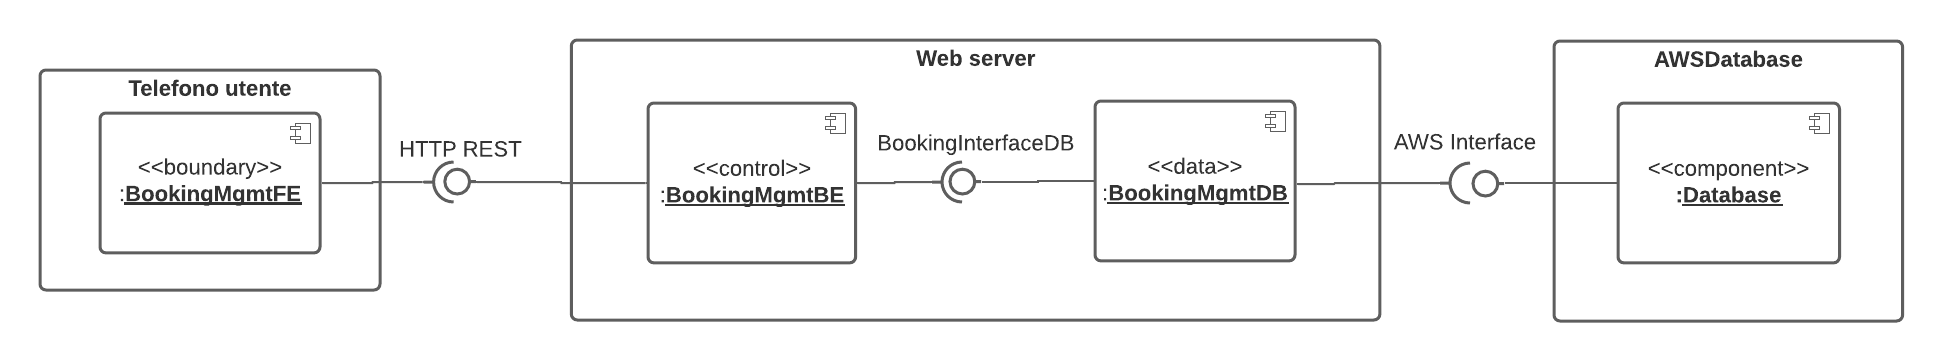
\includegraphics[width=\textwidth]{DeploymentDiagram2_v1.png}
    \caption{Deployment diagram UML.}\label{fig:DeploymentDiagram2}
\end{figure}